\only<beamer>{\titleframe}




\begin{frame}{Overview}
    \tableofcontents
\end{frame}




\sectionframe{Studium}

\section{Studium}

\begin{frame}{Lernorte}
    \begin{table}[h!]
	\centering
	\begin{tabular}{c|c|c}
	Ort & Vorteile  & Nachteile  \\ \hline \hline
	Universität & Geprüft & Dauer \\ \hline
	Autodidaktisch & Flexibler & Ungeprüft   \\ \hline
	Kurse & Reicht manchmal & Teuer   \\ \hline
	\end{tabular}
	\caption{Vergleiche von Lernorten}
	\label{tab:VergleichLernorte}
	\end{table}

\end{frame}


\begin{frame}{Coden lernen an der Universität Stuttgart}

    Das sind meine Kurse im ersten Semester:
    \begin{itemize}
        \item
        Mathematik für Informatiker
        \pause

        \item
        Programmierung und Software-Entwicklung
        \pause

        \item
        Programmentwicklung 
        \pause
        
        \item
        Bachelor Ringvorlesung
       
       
    \end{itemize}
\end{frame}



\sectionframe{Studienverlaufsplan}

\section{Studienverlaufsplan}

% text along an arrow
% (from LaTeX Stack Exchange: https://tex.stackexchange.com/a/154769,
% by Gonzalo Medina: https://tex.stackexchange.com/users/3954/gonzalo-medina,
% licensed under CC BY-SA: https://creativecommons.org/licenses/by-sa/3.0/)

\begin{frame}
\begin{figure}
\centering
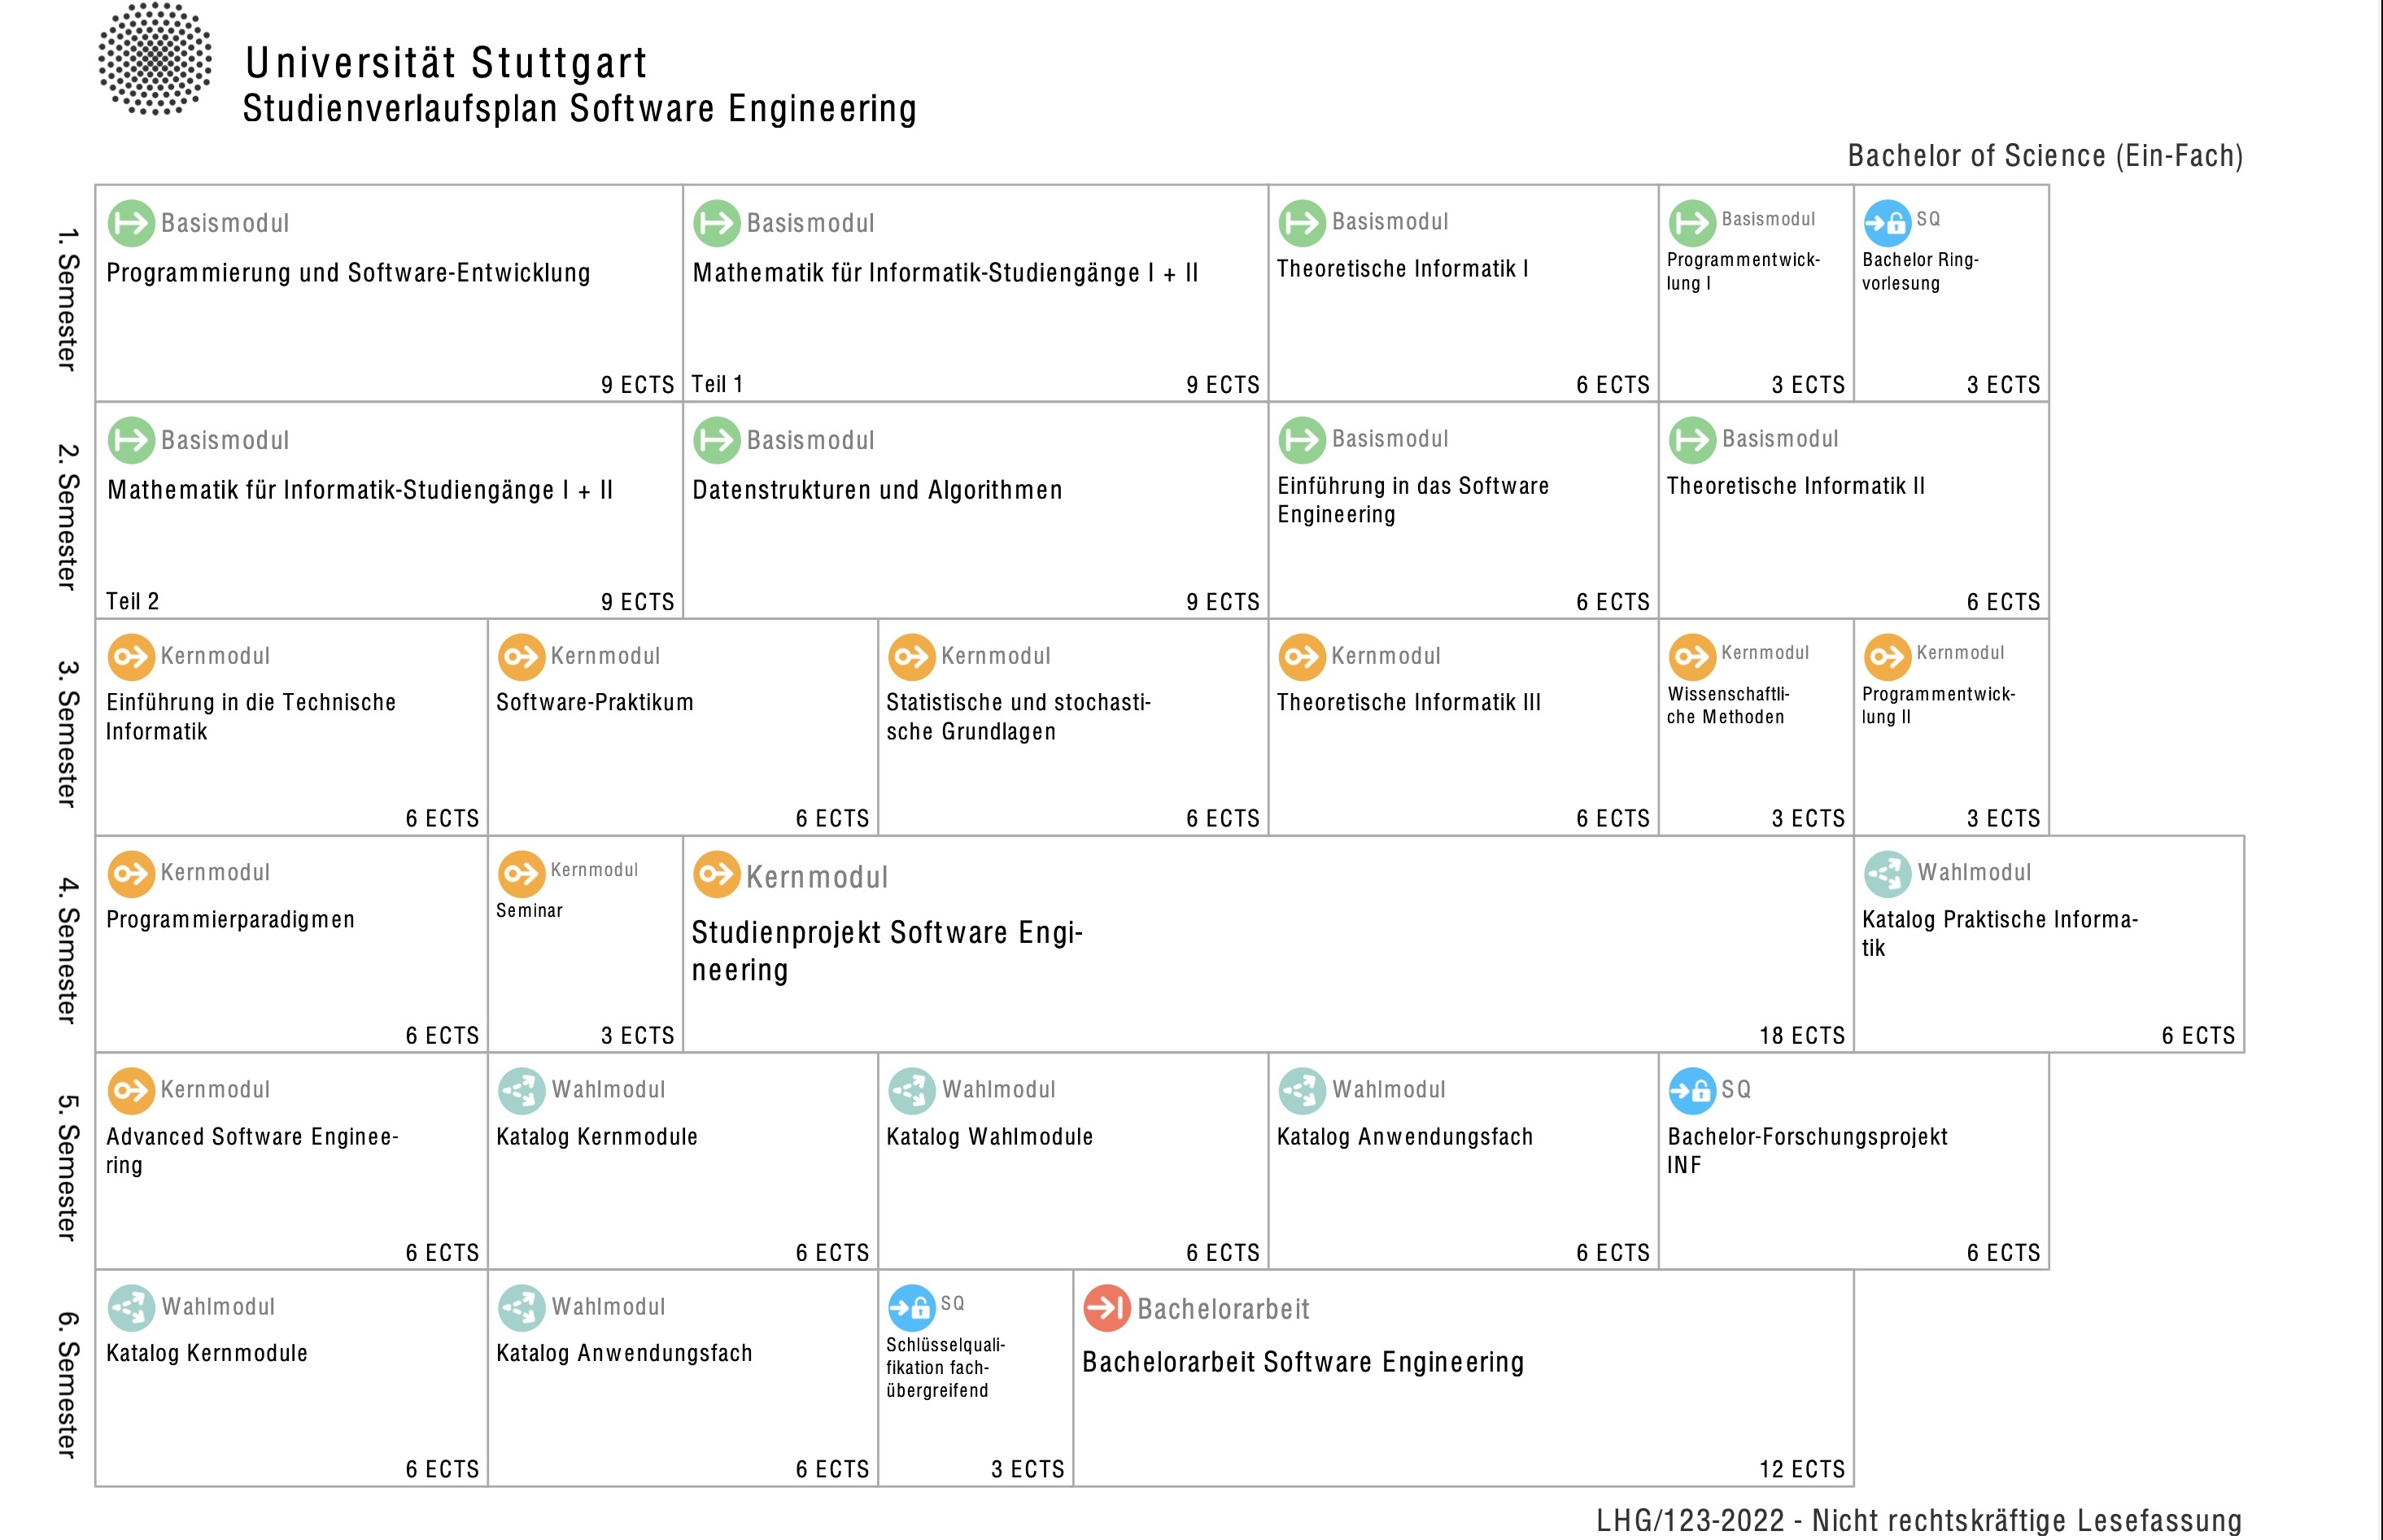
\includegraphics[width=0.75\textwidth]{studienplan.jpg}
\caption{Studienplan der Uni Stuttgart}
\label{fig:Studienplan}
\end{figure}
\end{frame}
